\documentclass{article}
\usepackage{iclr2027_conference,times}
\usepackage{amsmath,amssymb,graphicx,booktabs,microtype,xcolor}
\usepackage[utf8]{inputenc}
\usepackage{url}

% 待人工盲比回填的位置统一标记，避免漏改
\newcommand{\pending}[1]{\textcolor{red}{[PENDING: #1]}}

\title{When There Is No Right Answer:\\Evaluation Failure and a Sampling-Scale
Fix for Low-Resolution Pixel-Art Textures}

\author{Anonymous}

\begin{document}
\maketitle

\begin{abstract}
Low-resolution pixel-art texture generation exposes a blind spot in how
generative models are evaluated. When the output is a $16\times16$ grid of
discrete colour cells, independent artists drawing the \emph{same} material
agree on 9.8\% of cells against 8.6\% expected under a paired null
(50{,}753 artist pairs) --- there is no unique right answer. We show this
single fact breaks both mainstream automatic evaluation routes. Per-pixel
metrics measure marginal fit rather than quality. And VLM judges fail in ways
that per-item agreement cannot detect: on the same human-labelled set, two
judges agree with the human on \emph{identical} fractions of items
(66.7\%), yet one compresses an 86\% effect to 62\% ($p{=}0.14$) and erases
its stratification while the other preserves both; a third inverts the human
conclusion outright. Under human blind comparison a trivial downsampling
baseline beats a purpose-built masked-prediction model 83:17. The bottleneck
is not model capacity but a \emph{structural-unit convention} mismatch: the
generator draws ${\sim}25$ units per tile regardless of canvas while artists
draw ${\sim}4.5$, measured independently from 5{,}979 artist tiles and 125
artist sources. Cropping to the detected dominant period fixes it, and
manipulating the unit count produces a monotone dose--response in the fix's
benefit (88\%, 54\%, 17\% at 27.7, 13.8 and 9.4 units). We pre-registered and
\emph{falsified} a pure sampling-limit account along the way; reporting that
failure is what selects the surviving mechanism.
\end{abstract}

\section{Introduction}
\pending{prose; argument chain in docs/draft\_en.md \S1}

\section{Related Work}
\pending{prose; four-way positioning in docs/related-work.md}

\section{There Is No Right Answer}
\label{sec:noright}
\pending{3.1 agreement measurement, 3.2 per-pixel corollary, 3.3 judge failure}

\begin{figure}[t]
\centering
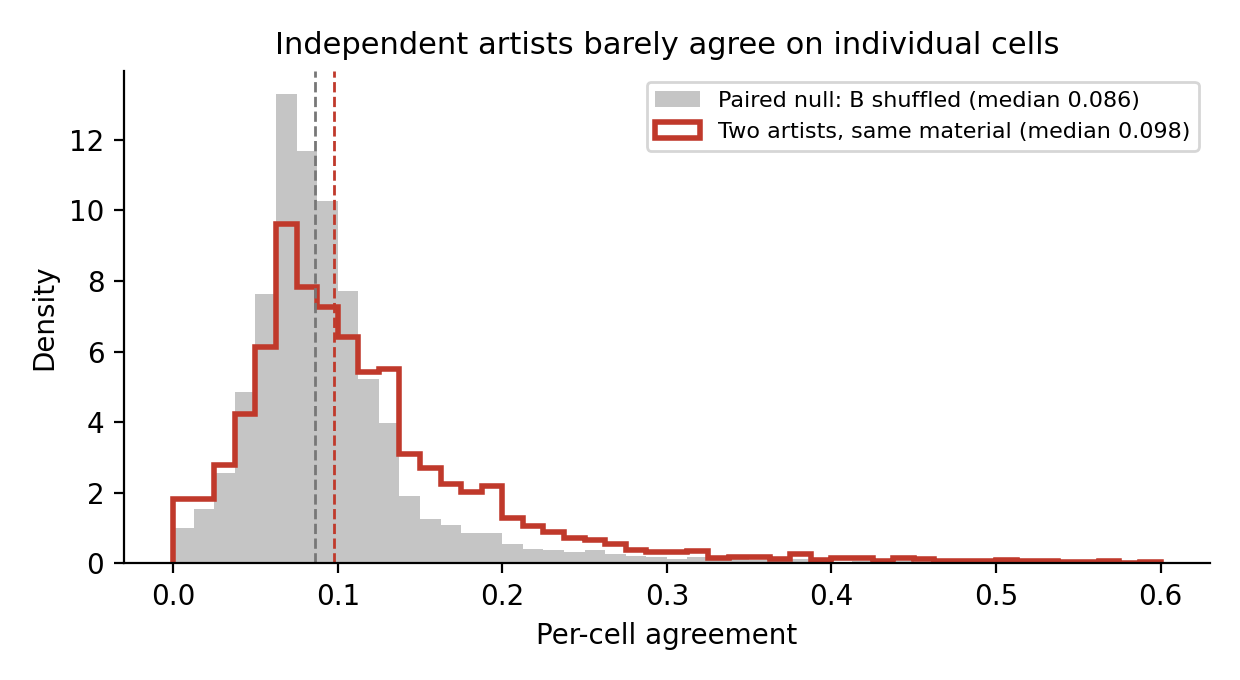
\includegraphics[width=.62\linewidth]{../figures/fig1_agreement.png}
\caption{Independent artists agree on individual cells barely above a paired
null. The null shuffles the second artist's own tile, preserving its marginal
while destroying its arrangement, so both sides pair the same marginals.}
\label{fig:agreement}
\end{figure}

\begin{figure}[t]
\centering
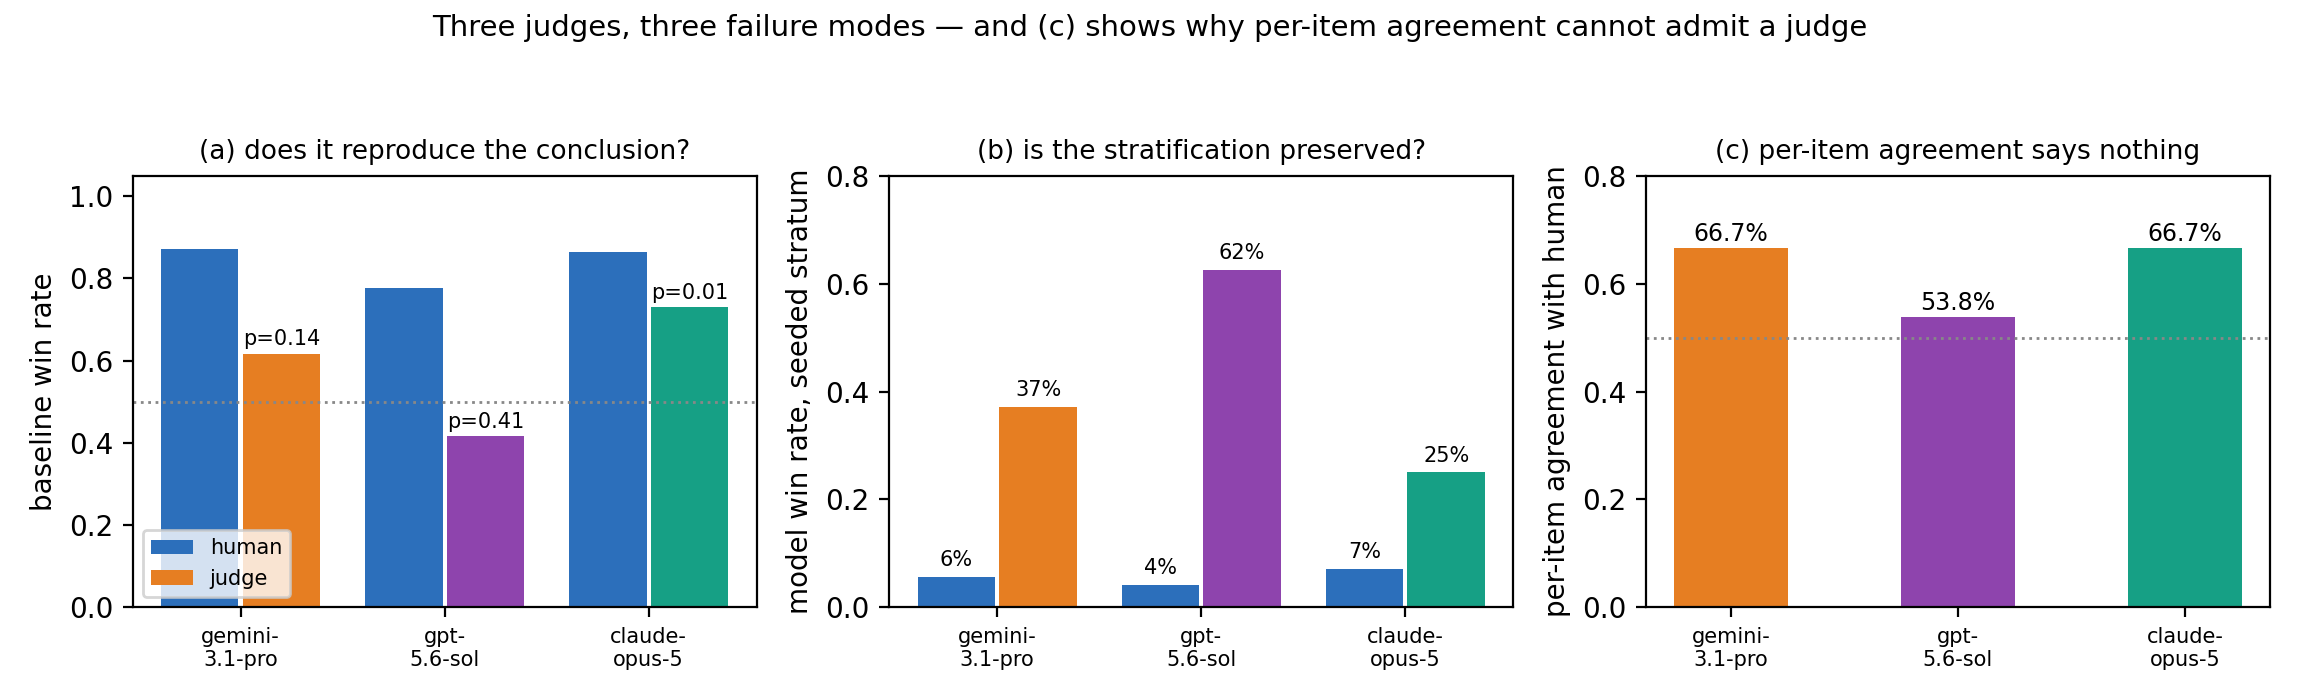
\includegraphics[width=\linewidth]{../figures/fig4_judges.png}
\caption{Three judges on the same human-labelled pairs. Panel (c) is the
methodological point: per-item agreement --- the quantity the VLM-as-judge
literature reports --- is identical for the judge that destroys the conclusion
and the one that preserves it.}
\label{fig:judges}
\end{figure}

\section{A Trivial Baseline Is Enough}
\pending{4.1 baseline vs artist, 4.2 baseline vs specialised model}

\section{The Real Bottleneck: Structural-Unit Convention}
\pending{5.1 diagnosis, 5.2 fix, 5.3 gate, 5.4 pre-registered falsification}

\begin{figure}[t]
\centering
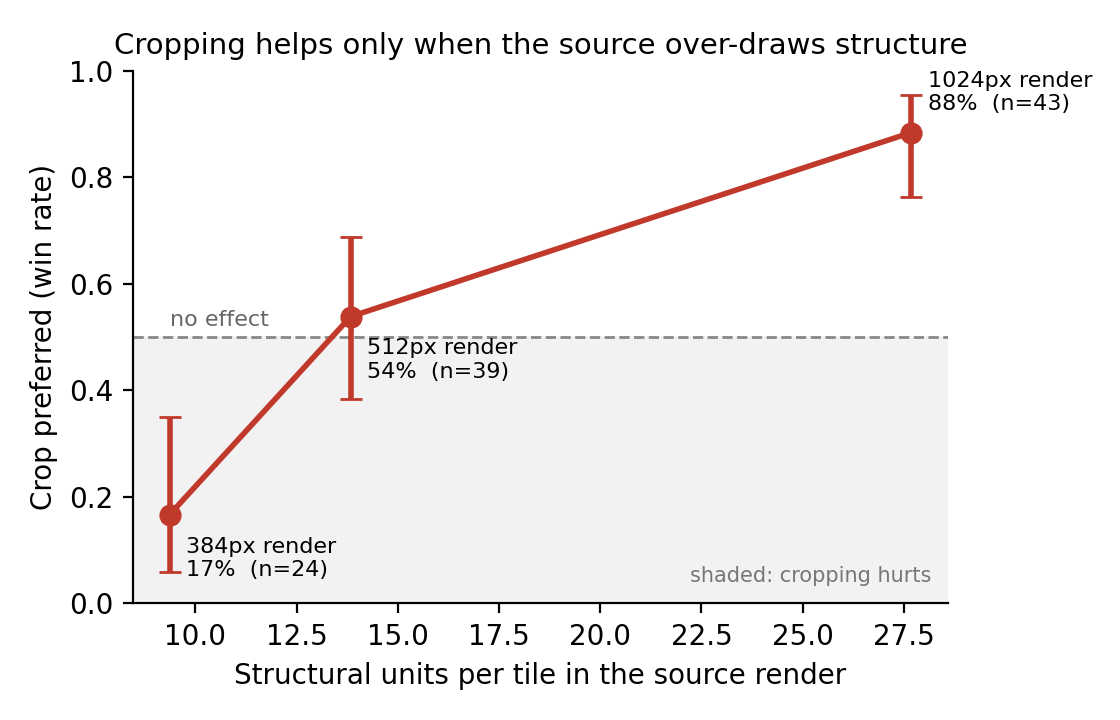
\includegraphics[width=.58\linewidth]{../figures/fig_dose_response.png}
\caption{Manipulating how many structural units the generator draws produces a
monotone change in whether cropping helps, with the midpoint sitting at no
effect. Bars are Jeffreys intervals.}
\label{fig:dose}
\end{figure}

\section{Limitations}
\pending{single annotator; 4.1 power; conditional win rates; per-image gate
does not follow from the condition-level effect}

\section*{Reproducibility Statement}
Every claim in this paper is traceable to a numbered experiment record in the
project log, including the six results we retracted. Pre-registrations are
git commits timestamped before the corresponding runs.

\bibliographystyle{iclr2027_conference}
\bibliography{refs}

\end{document}
